\section{Action\-Travel Class Reference}
\label{classActionTravel}\index{ActionTravel@{ActionTravel}}
Teleportation between maps action.  


{\tt \#include $<$actiontravel.hpp$>$}

Inheritance diagram for Action\-Travel::\begin{figure}[H]
\begin{center}
\leavevmode
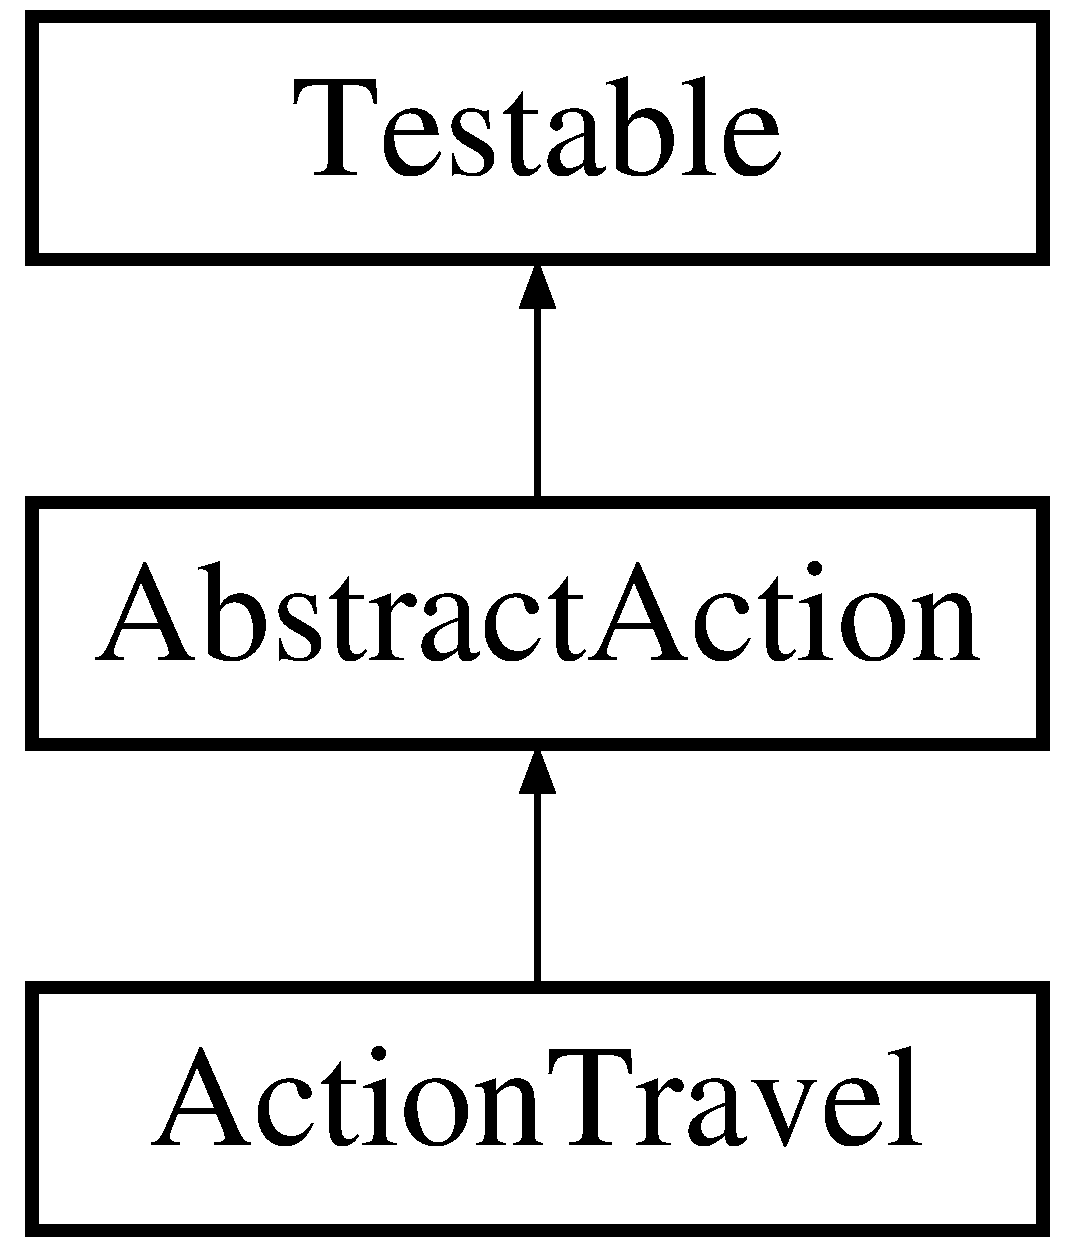
\includegraphics[height=3cm]{classActionTravel}
\end{center}
\end{figure}
\subsection*{Public Member Functions}
\begin{CompactItemize}
\item 
{\bf Action\-Travel} ({\bf Parser} \&parser)
\item 
bool {\bf run} ({\bf Monster} \&monster)
\item 
void {\bf load} ({\bf Parser} \&parser)
\item 
void {\bf save} (ofstream \&file)
\item 
int {\bf test} (bool verbose) const 
\end{CompactItemize}
\subsection*{Protected Attributes}
\begin{CompactItemize}
\item 
QString {\bf map\-Name}
\item 
{\bf Coordinates\-List} {\bf coordinates}
\end{CompactItemize}


\subsection{Detailed Description}
Teleportation between maps action. 



\subsection{Constructor \& Destructor Documentation}
\index{ActionTravel@{Action\-Travel}!ActionTravel@{ActionTravel}}
\index{ActionTravel@{ActionTravel}!ActionTravel@{Action\-Travel}}
\subsubsection{\setlength{\rightskip}{0pt plus 5cm}{\bf Action\-Travel} ({\bf Parser} \& {\em parser})}\label{classActionTravel_a0}




\subsection{Member Function Documentation}
\index{ActionTravel@{Action\-Travel}!load@{load}}
\index{load@{load}!ActionTravel@{Action\-Travel}}
\subsubsection{\setlength{\rightskip}{0pt plus 5cm}void load ({\bf Parser} \& {\em parser})\hspace{0.3cm}{\tt  [virtual]}}\label{classActionTravel_a2}




Implements {\bf Abstract\-Action} {\rm (p.\,\pageref{classAbstractAction_a2})}.\index{ActionTravel@{Action\-Travel}!run@{run}}
\index{run@{run}!ActionTravel@{Action\-Travel}}
\subsubsection{\setlength{\rightskip}{0pt plus 5cm}bool run ({\bf Monster} \& {\em monster})\hspace{0.3cm}{\tt  [virtual]}}\label{classActionTravel_a1}




Implements {\bf Abstract\-Action} {\rm (p.\,\pageref{classAbstractAction_a1})}.\index{ActionTravel@{Action\-Travel}!save@{save}}
\index{save@{save}!ActionTravel@{Action\-Travel}}
\subsubsection{\setlength{\rightskip}{0pt plus 5cm}void save (ofstream \& {\em file})\hspace{0.3cm}{\tt  [virtual]}}\label{classActionTravel_a3}




Implements {\bf Abstract\-Action} {\rm (p.\,\pageref{classAbstractAction_a3})}.\index{ActionTravel@{Action\-Travel}!test@{test}}
\index{test@{test}!ActionTravel@{Action\-Travel}}
\subsubsection{\setlength{\rightskip}{0pt plus 5cm}int test (bool {\em verbose}) const\hspace{0.3cm}{\tt  [virtual]}}\label{classActionTravel_a4}




Implements {\bf Testable} {\rm (p.\,\pageref{classTestable_a0})}.

\subsection{Member Data Documentation}
\index{ActionTravel@{Action\-Travel}!coordinates@{coordinates}}
\index{coordinates@{coordinates}!ActionTravel@{Action\-Travel}}
\subsubsection{\setlength{\rightskip}{0pt plus 5cm}{\bf Coordinates\-List} {\bf coordinates}\hspace{0.3cm}{\tt  [protected]}}\label{classActionTravel_p1}


\index{ActionTravel@{Action\-Travel}!mapName@{mapName}}
\index{mapName@{mapName}!ActionTravel@{Action\-Travel}}
\subsubsection{\setlength{\rightskip}{0pt plus 5cm}QString {\bf map\-Name}\hspace{0.3cm}{\tt  [protected]}}\label{classActionTravel_p0}




The documentation for this class was generated from the following files:\begin{CompactItemize}
\item 
{\bf actiontravel.hpp}\item 
{\bf actiontravel.cpp}\end{CompactItemize}
